\begin{Propriete}[Signe d'un trinôme]
    Soit $f$ la fonction polynôme de degré 2 définie sur $\R$ par $f(x)=a(x-x_1)(x-x_2)$ avec $a \neq 0$.
    
    Avec la convention $x_1 < x_2$, le tableau de signe de la fonction $f$ est donné par :
    
    \begin{center}
    \begin{tikzpicture}
    \tkzTabInit[espcl=3,lgt=2]{$x$/0.9,$f(x)$/0.9}
    {$-\infty$,$x_1$,$x_2$,$+\infty$}
    \tkzTabLine{,\text{signe de }a,z,\text{signe de }-a,z,\text{signe de } a}
    \end{tikzpicture}
    \end{center}
\end{Propriete}